%*******************************************************************************
%****************************** Second Chapter *********************************
%*******************************************************************************

\chapter{Second Chapter Title}
\label{chapter 2}
\ifpdf
    \graphicspath{{Chapter2/Figs/}{Chapter2/Figs/PDF/}{Chapter2/Figs/}}
\else
    \graphicspath{{Chapter2/Figs/Vector/}{Chapter2/Figs/}}
\fi
%********************************** % First Section  *************************************
\section{Basic Text and Refering Hints}
\LaTeX gives the possibility to bold a \textbf{word} or a \textbf{phrase containing more words} or mathematical equations like $\mathbf{A=B+C}$. \textit{Italic} and \underline{underline} commands are designed to be used in desired partof the text. Sizing the text is another optional command:
{\small Word}, {\large Word}, {\Large Word}.

%other options:
% \Huge
% \huge
% \LARGE
% \Large
% \large
% \normalsize (default)
% \small
% \footnotesize
% \scriptsize
% \tiny

Refering to the sections, chapters, equations and etc \dots is possible by command \verb|\ref{label}|. It is necessary to insert \verb|\label{name of section}| for each of desired section and chapter and etc \dots then refer them in any part of the text. For example in chapter \ref{chapter 1} we introduced the template and in section \ref{section 1.3} different folders and files in template were discribed. Figure \ref{fig:Greek} shows the greek letter codes in \LaTeX. 

Moreover in \LaTeX \footnote{Here there is the foot note explanation about the word \LaTeX} it is possible to have foot note explanation. You can also insert web links, if you do, make sure you use the full URL, including the \{http://\} for this. As an example by inserting the code: \begin{verbatim}
\href{http://www.polito.it}{polito website} \end{verbatim} you will have \href{http://www.polito.it}{polito website}. If you don't want to link URL and name, simply write the \verb|\url{http://www.polito.it}| and only romove the name. This is the result: (\url{http://www.polito.it}).

%********************************** % Second Section  *************************************
\section{Writing Mathematical Equations in \LaTeX} %Section - 2.2
\label{section 2.2}
% Uncomment this line, when you have siunitx package loaded.
%The SI Units for dynamic viscosity is \si{\newton\second\per\metre\squared}.
As an in-line equation example we can refer the most famous equation in the world: $E^2 = (m_0c^2)^2 + (pc)^2$, which is known as the \textbf{energy-mass-momentum} relation. You can write an equation in \textbf{equation} environment of \LaTeX, for example "Cauchy's Integral Formula" which is automatically given an equation number (tag) by \LaTeX{} like this:
\begin{verbatim}
\begin{equation}
CIF: \hspace*{5mm}F_0^j(a) =\frac{1}{2\pi \iota} \oint_{\gamma} 
\frac{F_0^j(z)}{z - a} dz
\end{equation}
\end{verbatim}
This will produce "Cauchy's Integral Formula" equation:

\begin{equation}
CIF: \hspace*{5mm}F_0^j(a) = \frac{1}{2\pi \iota} \oint_{\gamma} \frac{F_0^j(z)}{z - a} dz
\end{equation}

As you see the equation is tagged automatically according to the chapter and order. It is also possible to personalize tag for the equation:
\begin{equation}
\centering
\tag{Personalized tag}
CIF: \hspace*{5mm}F_0^j(a) = \frac{1}{2\pi \iota} \oint_{\gamma} \frac{F_0^j(z)}{z - a} dz
\end{equation}

\nomenclature[Z]{$CIF$}{Cauchy's Integral Formula}                                
% letter Z is for Acronyms 
\nomenclature[A]{$F$}{complex function}                                                  
%  letter A is for Roman symbols
\nomenclature[G]{$\pi$}{ $\simeq 3.14\ldots$}                                             
% letter G is for Greek Symbols
\nomenclature[G]{$\iota$}{unit imaginary number $\sqrt{-1}$}                      
% first letter G is for Greek Symbols
\nomenclature[G]{$\gamma$}{a simply closed curve on a complex plane}  
% first letter G is for Greek Symbols
\nomenclature[X]{$\oint_\gamma$}{integration around a curve $\gamma$} 
% first letter X is for Other Symbols
\nomenclature[R]{$j$}{superscript index}                                                       
% first letter R is for superscripts
\nomenclature[S]{$0$}{subscript index}
% first letter S is for subscripts

To make the \textbf{Nomenculature } you need to Issue the \verb|\nomenclature| command for each symbol you want to have included in the nomenclature list. The best place for this command is immediately after you introduce the symbol for
the first time. For the equation above:

\begin{verbatim}
\nomenclature[Z]{$CIF$}{Cauchy's Integral Formula}                                
\nomenclature[A]{$F$}{complex function}                                                  
\nomenclature[G]{$\pi$}{ $\simeq 3.14\ldots$}                                             
\nomenclature[G]{$\iota$}{unit imaginary number $\sqrt{-1}$}                      
\nomenclature[G]{$\gamma$}{a closed curve on a complex plane}  
\nomenclature[X]{$\oint_\gamma$}{integration around a curve 
$\gamma$} 
\nomenclature[R]{$j$}{superscript index}                                                       
\nomenclature[S]{$0$}{subscript index}
%letter Z is for Acronyms, A is for Roman symbols, G is for Greek 
Symbols, X is for Other Symbols letter, R is for superscripts, S 
is for subscripts
\end{verbatim}

To make nomenclature list you need to run "pdflatex" for \textbf{.tex} file and then run the "makeindex" command and then again run "pdflatex" for \textbf{.tex} file. (make sure in "Options> Configurations >Commands >make index" box there is "makeindex -s nomencl.ist -t \%.nlg -o \%.nls \%.nlo", if not, just copy and paste this command in the box and follow the instruction above).


If there are several equations that you need to align vertically, the \textbf{align} environment will do it:
\begin{align*}
	x&=5y           &  w &=-z              &  a&=b-c\\
	2x&=-y         &  3w&=\frac{1}{2}z   &  a&=3b\\
	-4 + 5x&=2+y   &  w+2&=-1+w          &  ab&=\frac{-1}{3}cb
\end{align*}

%using * will remove the tags from equations.

\vspace{0.5cm}

%********************************** % Third Section  ***************************
\section{List Formatting in \LaTeX}
\label{section 2.3}
Convenient and predictable list formatting is one of the many advantages of using \LaTeX . Latex distinguishes between three different enumeration/itemization environments: 
%
\begin{itemize}
	\item Enumerate for an enumerated list,
	\item Itemize for a bullet list,
	\item Description for a descriptive list.
\end{itemize}
All lists follow a basic format and each of them provide four levels, which means you can have nested lists of up to four levels.

\subsection{Enumerate}

\begin{enumerate}
	\item The first topic is "Good"
	\item The second topic is "Intermediate" (Lev. 1)
	\begin{enumerate}
		\item The first subtopic is "high intermediate"
		\item The second subtopic is "low intermediate"(Lev. 2)
		\begin{enumerate}
			\item The first subsubtopic is "very low intermediate"(Lev. 3)
			\begin{enumerate}
				\item The first subsubsubtopic is "too low intermediate"(Lev. 4)
			\end{enumerate}
		\end{enumerate}
	\end{enumerate}
	\item The third topic is "Bad"
\end{enumerate}
 

\subsection{Itemize}

\begin{itemize}
	\item The first topic is "Good"
    \item The second topic is "Intermediate"
    \begin{itemize}
	     \item The first subtopic is "high intermediate"
	     \item The second subtopic is "low intermediate"
	     \begin{itemize}
		      \item The first subsubtopic is "very low intermediate"
	     \end{itemize}
\end{itemize}
\item The third topic is "Bad"
\end{itemize}

\subsection{Description}
\begin{description}
	\item [The first topic] is "Good"
    \item [The second topic] is "Intermediate"
    \begin{description}
	      \item [The first subtopic] is "high intermediate"
	      \item [The second subtopic] is "low intermediate"
	      \begin{description}
		        \item [The first subsubtopic] is "very low intermediate"
	      \end{description}
\end{description}
\item [The third topic] is "Bad"
\end{description}


%********************************** % Forth Section  ***************************

\section{Figures}
\label{section 2.4}
There will hopefully be many figures in your thesis (that should be placed in the \textbf{Figs} folder in each chapter folder). The way to insert figures into your thesis is to use a code template like this:
\begin{verbatim}
\begin{figure}[H] 
\centering    
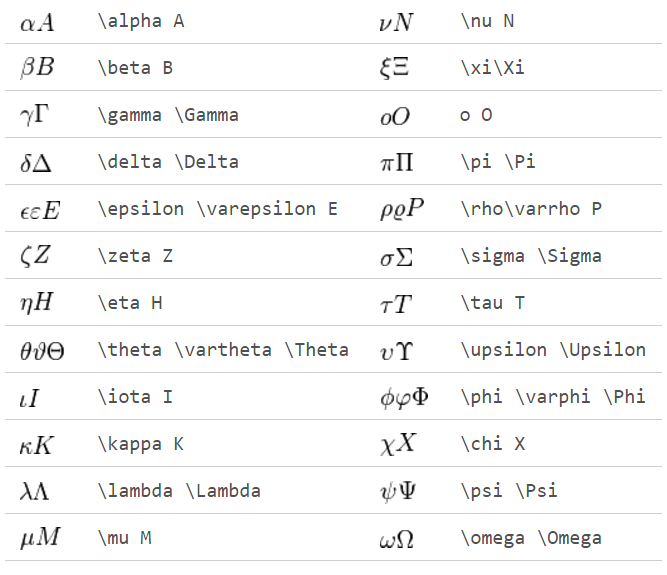
\includegraphics[width=1.0\textwidth]{Greek_letters}
\caption[Greek letters in latex]{List of greek letters in Latex}
\label{fig:Greek}
\end{figure}
\end{verbatim}
Also look in the source file. Putting this code into the source file produces the Figure~\ref{fig:Greek} that you can see in the figure below. By changing the value of figure width (\verb|width=1.0\textwidth|) you can change the figure dimension.

\begin{figure}[H] 
\centering    
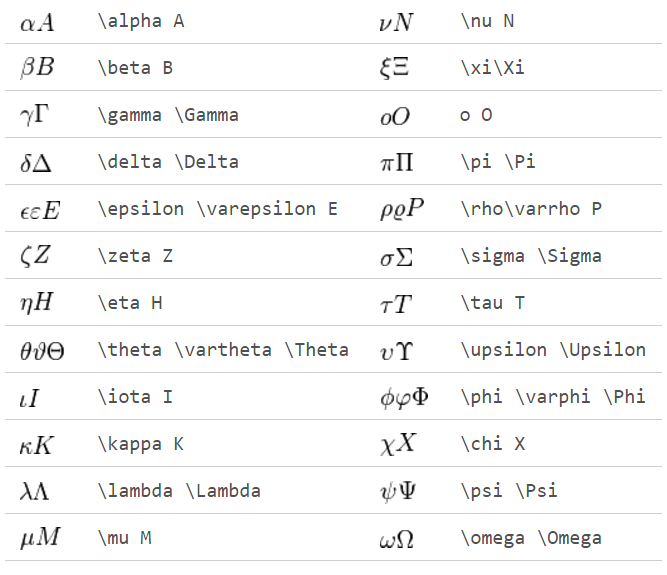
\includegraphics[width=0.8\textwidth]{Greek_letters}
\caption[Greek letters in latex]{List of greek letters in Latex}
\label{fig:Greek}
\end{figure}


\begin{landscape}

\section*{Subplots}
The multiple figure example in landscape form is presented here. Here you can refer any subfigure for example  arrows (see Fig.~\ref{fig:Arrows}) and binary operation symbols in (Fig.~\ref{fig:Miscsymb}) or you can cite the whole figure as Fig.~\ref{fig:Mathsymb}


\begin{figure}
  \centering
  \begin{subfigure}[b]{0.5\textwidth}
    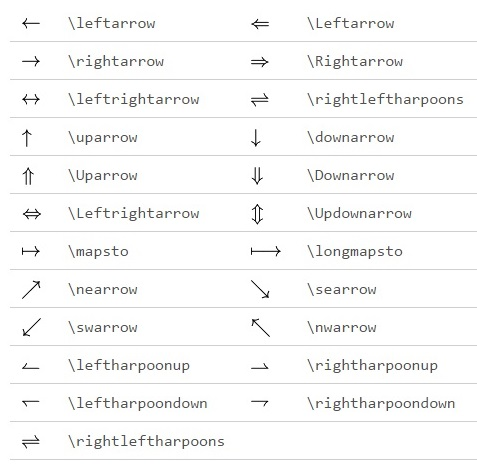
\includegraphics[width=\textwidth]{Arrows}
    \caption{Arrows}
    \label{fig:Arrows}   
  \end{subfigure}             
  \begin{subfigure}[b]{0.5\textwidth}
    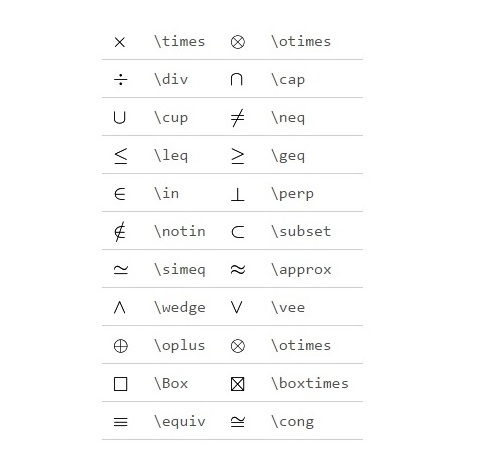
\includegraphics[width=\textwidth]{Binary_operations}
    \caption{Binary operations symbols}
    \label{fig:Binarysymb}
  \end{subfigure}             
  \begin{subfigure}[b]{0.5\textwidth}
    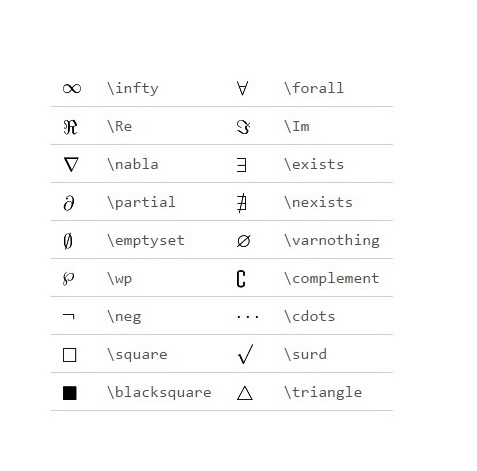
\includegraphics[width=\textwidth]{Miscellaneous_symbols}
    \caption{Miscellaneous sybols}
    \label{fig:Miscsymb}
  \end{subfigure}
  \caption{Useful math symbols in Latex}
  \label{fig:Mathsymb}
\end{figure}

\end{landscape}

%********************************** % Fifth Section  ***************************
\section{Tables}

The layout of a table has been established over centuries of experience and 
should only be altered in extraordinary circumstances \cite{fear2005publication}. 

When formatting a table, remember two simple guidelines at all times:

\begin{enumerate}
	\item Never, ever use vertical rules (lines).
	\item Never use double rules.
\end{enumerate}

These guidelines may seem extreme but I have
never found a good argument in favour of breaking them. For
example, if you feel that the information in the left half of
a table is so different from that on the right that it needs
to be separated by a vertical line, then you should use two
tables instead. Not everyone follows the second guideline:

There are three further guidelines worth mentioning here as they
are generally not known outside the circle of professional
typesetters and subeditors:
\begin{enumerate}\setcounter{enumi}{2}
	\item Put the units in the column heading (not in the body of
	the table).
	\item Always precede a decimal point by a digit; thus 0.1
	{\em not} just .1.
	\item Do not use `ditto' signs or any other such convention to
	repeat a previous value. In many circumstances a blank
	will serve just as well. If it won't, then repeat the value.
\end{enumerate}
A frequently seen mistake is to use `\textbackslash begin\{center\}' \dots `\textbackslash end\{center\}' inside a figure or table environment. This center environment can cause additional vertical space. If you want to avoid that just use `\textbackslash centering'

\begin{table}
	\caption{A badly formatted table}
	\centering
	\label{table:bad_table}
	\begin{tabular}{|l|c|c|c|c|}
		\hline 
		& \multicolumn{2}{c}{Species I} & \multicolumn{2}{c|}{Species II} \\ 
		\hline
		Dental measurement  & mean & SD  & mean & SD  \\ \hline 
		\hline
		I1MD & 6.23 & 0.91 & 5.2  & 0.7  \\
		\hline 
		I1LL & 7.48 & 0.56 & 8.7  & 0.71 \\
		\hline 
		I2MD & 3.99 & 0.63 & 4.22 & 0.54 \\
		\hline 
		I2LL & 6.81 & 0.02 & 6.66 & 0.01 \\
		\hline 
		CMD & 13.47 & 0.09 & 10.55 & 0.05 \\
		\hline 
		CBL & 11.88 & 0.05 & 13.11 & 0.04\\ 
		\hline 
	\end{tabular}
\end{table}

\begin{table}
	\caption{A nice looking table}
	\centering
	\label{table:nice_table}
	\begin{tabular}{l c c c c}
		\hline 
		\multirow{2}{*}{Dental measurement} & \multicolumn{2}{c}{Species I} & \multicolumn{2}{c}{Species II} \\ 
		\cline{2-5}
		& mean & SD  & mean & SD  \\ 
		\hline
		I1MD & 6.23 & 0.91 & 5.2  & 0.7  \\
		
		I1LL & 7.48 & 0.56 & 8.7  & 0.71 \\
		
		I2MD & 3.99 & 0.63 & 4.22 & 0.54 \\
		
		I2LL & 6.81 & 0.02 & 6.66 & 0.01 \\
		
		CMD & 13.47 & 0.09 & 10.55 & 0.05 \\
		
		CBL & 11.88 & 0.05 & 13.11 & 0.04\\ 
		\hline 
	\end{tabular}
\end{table}


\begin{table}
	\caption{Even better looking table using booktabs}
	\centering
	\label{table:good_table}
	\begin{tabular}{l c c c c}
		\toprule
		\multirow{2}{*}{Dental measurement} & \multicolumn{2}{c}{Species I} & \multicolumn{2}{c}{Species II} \\ 
		\cmidrule{2-5}
		& mean & SD  & mean & SD  \\ 
		\midrule
		I1MD & 6.23 & 0.91 & 5.2  & 0.7  \\
		
		I1LL & 7.48 & 0.56 & 8.7  & 0.71 \\
		
		I2MD & 3.99 & 0.63 & 4.22 & 0.54 \\
		
		I2LL & 6.81 & 0.02 & 6.66 & 0.01 \\
		
		CMD & 13.47 & 0.09 & 10.55 & 0.05 \\
		
		CBL & 11.88 & 0.05 & 13.11 & 0.04\\ 
		\bottomrule
	\end{tabular}
\end{table}
